\nnarticleheader{tDCS and rTMS: Promising Treatments for Alzheimer’s Disease}{Carson DeMarco, Haverford '20}
What disease currently stands as the sixth leading cause of death in the United States, yet has no cure? Alzheimer’s Disease (AD). By the year 2050, 5.8 million Americans are projected to be diagnosed with AD. Additionally, AD is a heavy financial burden and will cost the United States 290 billion dollars for continued treatment by 2050 \cite{Association}. AD, which primarily affects memory, is a harmful neurodegenerative disease, an irreversible condition leading to gradual degeneration or death of nerve cells in the central nervous system (CNS) \cite{JNPD}. The CNS, which integrates and processes information from the sensory division of the peripheral nervous system, is vital for the human body to function normally, and the malfunction of this system lead to detrimental health issues. While AD remains incurable, two current treatments have proven to enhance cognitive thinking and memory: Transcranial Direct Current Stimulation and Repetitive Transcranial Magnetic Stimulation.

AD disrupts the communication between neurons and kills them. AD first targets and destroys neurons in the brain associated with memory, such as those found in the cerebral cortex (the brain’s memory center) and the entorhinal cortex (the network in the brain for memory, perception of time, and navigation). Additionally, AD targets the hippocampus, the brain region that turns short-term memories into long-term memories. In later stages, AD affects more regions in the cerebral cortex, such as the prefrontal cortex, the center for cognitive thinking and decision making. Symptoms of these later stages include the inability to perform normal daily tasks, such as driving, reading, and communicating. In the final stages of AD, known as brain atrophy, the brain loses volume: enough neurodegeneration has occurred to an extent that the brain actually shrinks in size \cite{Health}.

The emergence of AD is caused by two main issues: Beta-Amyloid Plaques and Neurofibrillary Tangles. Beta-Amyloid Plaques arise by the accumulation of a malformed protein called Amyloid-Beta Precursor Protein (APP) in the cerebrospinal fluid. APP is a transmembrane protein vital for neural growth and repair. A small peptide from this protein can branch-off and leave the membrane, where it changes shape and aggregates into larger molecules, causing plaque formation near the cells \cite{Goodsell}. The Neurofibrillary Tangles emerge from an abnormal version of a protein called Tau. This protein helps to form microtubules, structures that facilitate the transportation of nutrients and essential molecules to different parts in the cell. Abnormal versions of this protein arise when misfolding occurs during protein expression, and a “loose end” sticks out, recruiting more abnormal Tau proteins to attach, leading to the formation of tangles inside the cells. Consequently, the tangles inhibit the neuron from performing normal intracellular functions \cite{Foundation}. Between the two primary factors that lead to AD, the neurons lose their ability to communicate; their dendrites, extensions from the cell that transfer signals, retract and neural connections are lost, leading to neurodegeneration, eventual cell death, and brain shrinkage \cite{Health}. Transcranial Direct Current Stimulation, however, has demonstrated the ability to improve these connections and alleviate the experienced symptoms of AD.

\renewcommand{\thefigure}{1}
\begin{wrapfigure}{R}{0.5\textwidth}
  \begin{center}
    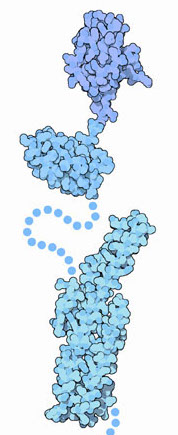
\includegraphics[width=0.26\textwidth]{demarco_app}
  \end{center}
  \caption{A molecular representation of APP}
\end{wrapfigure}

Transcranial Direct Current Stimulation (tDCS) serves as a non-invasive brain stimulation technique shown to improve cognitive abilities and memory associations for individuals affected by Alzheimer’s. tDCS modulates the excitability of a specific brain region by changing the membrane potential, the difference in charge between the inside of a neuron (negatively charged) and the outside of a neuron (positively charged), and modifies the brain circuitries. tDCS has become more prevalent for Alzheimer’s treatment since it promotes neuromodulation, the regulation of controlling neurotransmitters, and cortical changes, improved cognitive functioning. tDCS sends an electrical current across specific brain regions by placing two electrodes on the scalp of the head and has demonstrated improvement in cognitive ability for patients in conducted studies \cite{Machado}.

One study used tDCS for patients with AD to improve their ability to associate pictures with their names. Over the course of ten sessions with 30 minutes of anodal tDCS, a type of tDCS stimulation that excites neural activity, applied to the parietal lobe. The parietal lobe includes brain regions associated with reception and correlation of sensory information. The patients were trained to associate pictures with their corresponding names to show improvements in their cognitive thinking and memory. Several evaluations were conducted: before stimulation, after stimulation, two weeks post-stimulation, and two months post-stimulation. Analysis of the evaluations indicated significant improvements in the patient’s abilities to associate a picture by its name after tDCS. Additional analysis of the parietal lobe after stimulation showed continued improvement beyond the two months post-stimulation evaluation. Thus, tDCS has demonstrated promise to potentially reverse the effects of AD \cite{Chertkow}.

Similarly to tDCS, Repetitive Transcranial Magnetic Stimulation (rTMS) is a non-invasive brain stimulation technique that induces electrical currents based on the principle of electromagnetic induction, the production of an electromotive force across an electrical conductor in a changing magnetic field. The magnetic field is generated by a strong current  circulating within a coiled position in the brain, creating an electrical current through the cortical tissue underneath the coil, delivering rhythmic and repetitive pulses to modulate neural activity. High-frequency rTMS stimulates neural activity, and observations have indicated this stimulation produces positive effects in the brain, such as inducing Long-Term Potentiation (LTP), the consistent strengthening of neural synapses. Several recent clinical trials were conducted to determine the efficacy and safety of rTMS for patients with AD, and the trials presented positive outcomes in cognitive functioning \cite{Dong}.

Alzheimer’s Disease is a deadly neurodegenerative disease. Current promising treatments include the Transcranial Direct Current Stimulation and Repetitive Transcranial Magnetic Stimulation, both non-invasive brain stimulation techniques that are effective for enhancing cognitive function and memory associations damaged by AD. Further and future research into Alzheimer’s should be focused on finding ways to clear and remove the Beta-Amyloid Plaques and Neurofibrillary Tangles in the CNS, not only restoring the health of the affected neurons, but also the health of individuals impacted by the disease.

\newpage
\noindent
\textbf{References}
\begingroup
\renewcommand{\section}[2]{}% https://tex.stackexchange.com/questions/22645/hiding-the-title-of-the-bibliography
%\renewcommand{\chapter}[2]{}% for other classes
\begin{thebibliography}{9}
\bibitem{Alzheimer's}
Alzheimer's, U. A. (2019). The Alzheimer's Crisis. Retrieved January 13, 2020, from
\url{https://www.usagainstalzheimers.org/learn/alzheimers-crisis?gclid=EAIaIQobChMInNS
zrHr5gIVBqSzCh3ykgOpEAAYBCAAEgInD_D_BwE}.

\bibitem{Association}
Association, A. (n.d.). Facts and Figures. Retrieved January 15, 2020, from
\url{https://www.alz.org/alzheimers-dementia/facts-figures}.

\bibitem{Chertkow}
Chertkow, H., Roncero, C., Kneifel, H., Thiel, A., Probst, S., Malus, M., and Solomon, S. (2017,
April 18). Transcranial direct current stimulation (tDCS) improves picture naming in
Alzheimer's Disease and Frontotemporal dementia. (P3.089). \textit{Neurology}. Retrieved January 15, 2020, from \url{https://n.neurology.org/content/88/16_Supplement/P3.089}.

\bibitem{Dong}
Dong, X., Yan, L., Huang, L., \textit{et al}. (2018, October 12).
Repetitive transcranial magnetic stimulation for the treatment of Alzheimer's disease: A
systematic review and meta-analysis of randomized controlled trials. \textit{PLOS}. Retrieved January
15, 2020, from \url{https://journals.plos.org/plosone/article?id=10.1371/journal.pone.0205704}.

\bibitem{Foundation}
Foundation, B. F. (2019, December 11). Amyloid Plaques and Neurofibrillary Tangles. Retrieved
January 14, 2020, from \url{https://www.brightfocus.org/alzheimers-disease/infographic/amyloid-plaques-and-neurofibrillary-tangles}.

\bibitem{Goodsell}
Goodsell, D. (2006, July). PDB101: Molecule of the Month: Amyloid-beta Precursor Protein.
Retrieved January 14, 2020, from \url{https://pdb101.rcsb.org/motm/79}.

\bibitem{Health}
Health, N. I. of. (n.d.). What Happens to the Brain in Alzheimer's Disease? National Institute on
Aging. Retrieved January 13, 2020, from \url{https://www.nia.nih.gov/health/what-happens-brain-alzheimers-disease}.

\bibitem{JNPD}
JNPD, Research (Ed.). (2019). What is Neurodegenerative Disease? Retrieved January 13, 2020, 
from \url{https://www.neurodegenerationresearch.eu/about/what/}.

\bibitem{Machado}
Machado, S. (2016, September 30). Transcranial Direct Current Stimulation as a Potential Tool
for Cognitive Rehabilitation on Alzheimer's Disease. \textit{Clinical Psychiatry}. Retrieved January 15, 2020, from
\url{http://clinical-psychiatry.imedpub.com/transcranial-direct-current-stimulation-as-a-potential-tool-for-cognitive-rehabilitation-on-alzheimers-disease.php?aid=17213}.

\end{thebibliography}
\endgroup